\chapter{Implementation}
\label{chaptImplementation}
In this chapter, we describe the implementation of our demonstration game and explain the basic principles and algorithms behind it. Then we present measurements of performance of main algorithms used in the implementation.

At first, we considered implementation based on \emph{A fast method for simulating destruction and the generated dust and debris} (FMSDGDD) (see \cref{sec:edem}). However, after degrading performance issues~\cref{sec:testing} we decided to abandon this approach.

After consideration of various approaches implemented in games and also proposed efficient solutions to the problem of real-time destructible environment, we decided to implement and test an approach based on \emph{Geomod} (described in \cref{sec:common}) technique. The \emph{Geomod} inspired us to create object representing empty space and use boolean subtraction operation on the mesh to generate damaged body. Abandoned FMSDGDD approach influenced us to generate debris equivalent to the removed volume and use boolean intersection. We implemented this idea by using an intersection of \emph{Geomod} inspired empty space and original mesh as a debris.

\section{Main algorithm}
As mentioned, our algorithm uses boolean operations similarly to \emph{Geomod}s removal of an empty space from the terrain. The difference is that we apply this method to rigid body objects and permanently alter their mesh. The shape of removed object is determined by Voronoi cell that is generated dynamically for every collision. The collision information is received from the physics engine.

Our approach generates Voronoi cell at the point of collision. The decision to use one cell instead of a fracture pattern, like the one described in Real Time Dynamic Fracture with Volumetric Approximate Convex Decompositions algorithm (see \cref{sec:RTDF}), is based on the fact that we want to observe how dependent is our design on the complexity of destructed objects and not on the complexity of fracture pattern. Our implementation is easily expandable to the use of multiple cells or cells of any shape. 

After the cell generation, the difference of original mesh and the Voronoi cell is calculated to represent the damaged objects. To generate the debris, the intersection of original mesh and the Voronoi cell is calculated. This action effectively cuts the object into two or more pieces, all of which are put back into simulation and can be damaged again (see \cref{fig:subtraction}). The Voronoi cell was chosen because it has easily randomizable shape and provides aesthetically good results.

The cost of fracturing in our implementation is solely dependent on the size and complexity of the fractured object~\cref{sec:testing}. This makes the method suitable for use in computer games with a large number of simple objects with low polygon meshes.

\begin{figure}
        \centering
        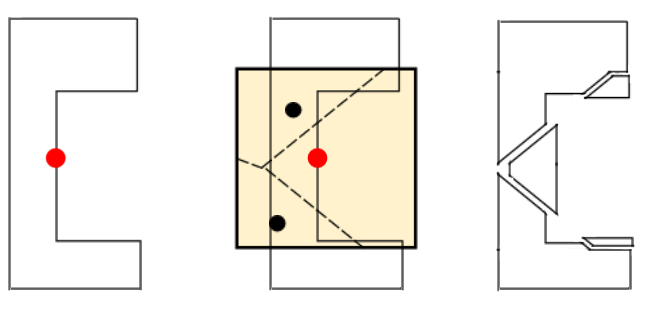
\includegraphics[width=\textwidth]{img/subtractionProcess}
        \caption{object with point of collision (left), generated Voronoi cells (centre), object divided into five new smaller objects after subtraction of the Voronoi cell belonging to the point of collision (right)}
        \label{fig:subtraction}
\end{figure}

To generate the Voronoi cell, we create a closed domain with the centre at the point of collision. In the domain, we need to create random points so the Voronoi cell of the point of collision does not cover entire domain. This step also ensures variability of generated cells. After that, we can use a Voronoi cell belonging to the point of collision as the object we subtract from the object being damaged. The boundaries of the domain clip the generated Voronoi cell, therefore the Voronoi cell can never be larger than the domain. Randomization of the size and shape of a Voronoi cell guarantees different result after every damage application.

\section{Program Structure}
The main program loop runs in following steps:
\begin{enumerate}
\item Perform a step in physics simulation.\todo{Tohle je spatny. Kde je definovanej `step in physics simulation'? K popisu vsech algoritmu je potreba mit aspon ramcove popsany data co jdou dovnitr, co to s nima (proc) udela, a kam jdou ven.}
\item Handle collisions and perform destruction, as described in  \cref{sec:collisions}.
\item Read user input and then apply correct forces to the controlled vehicle.
\item Render the current state of objects. In this step, a graphical representation of every object is updated to comply with its rigid body version.
\end{enumerate}

\begin{figure}
        \centering
        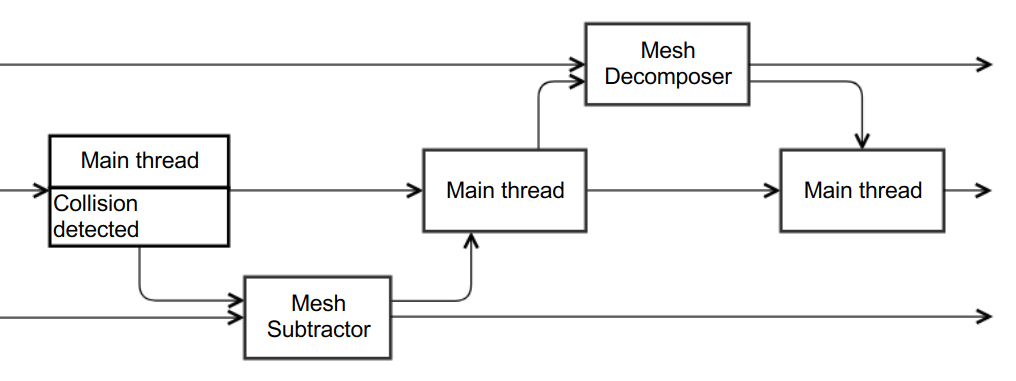
\includegraphics[width=\textwidth]{img/decompositionFlow}
        \caption{Diagram is showing multiple threads handling collision event. }
        \label{fig:threads}
\end{figure}

We want to keep a constant frame-rate in our application, but we do not  expect the mesh subtraction and convex decomposition tasks to perform in required time and therefore we execute them asynchronously in separate threads. As a result, the program is running in three threads (\cref{fig:threads}): the main thread, a thread for subtracting meshes and a thread for decomposing triangular mesh into a set of convex shapes (\cref{sec:decomposition}). Both subtraction and decomposition threads communicate solely with the main thread, and all communication is done in producer-consumer model. Figure \ref{fig:objectInThreads} shows the changes of the object and its collision shape across all threads.

We use only one thread for all mesh subtraction tasks because we anticipate that the most of the consecutive collisions are going to be triggered by the same object --- shooting at one building multiple times in a row. In this situation, one subtraction does not have valid input data until the previous one has finished, which leads to sequential processing. If we were to expect the collision occurring randomly on independent objects we could implement a thread pool for resolving subtraction tasks. When processing multiple collisions on the same object with multiple threads, the order of applying subtraction is not important as long as all tasks are processed and applied. Multiple thread solution would require implementation of a locking mechanism to avoid race conditions.

A use of a larger thread pool could be useful for convex decomposition. With multiple threads, the object could have been changed since the current calculation started. This conflicting state means we can not apply the current result but we know for sure that another decomposition task was created when the change occurred. We do not know whether the newer task has already finished or not, but we know for certain, that if we discard our decomposition, the object has either temporary shape or a new valid decomposition. We did not implement a thread pool solution because we did not see it necessary and our hardware \todo{current common gaming hardware, citation needed} is not well suited for running more than four simultaneous threads.

\begin{figure}
        \centering
        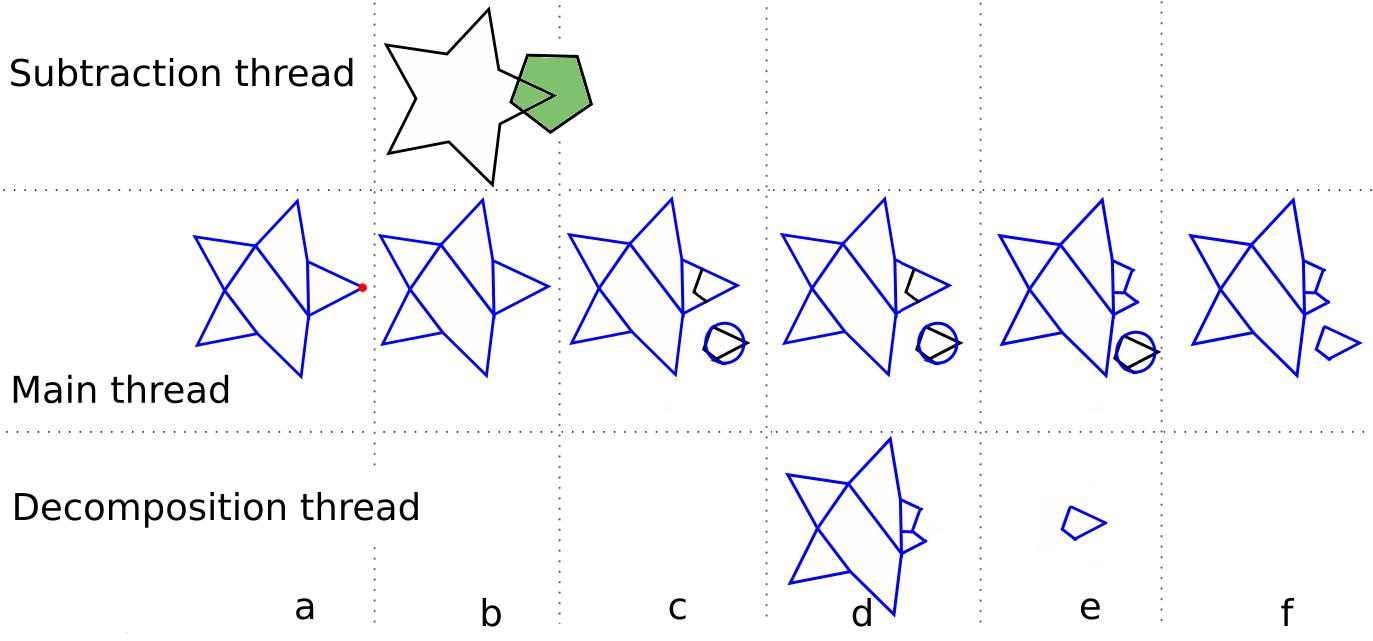
\includegraphics[width=\textwidth]{img/object-progress}
       \caption{Simplified overview of collision handling across multiple threads in simultaneous time slots. (a): collision was detected (red), (b): Voronoi cell (green) is being subtracted from the original mesh (black) in subtraction thread, (c): the result of the subtraction are two objects --- one one without change in collision shape (blue) and one with temporary spherical shape, (d) and (e): new collision shapes are computed in decomposition thread, (f): the final result.}
        \label{fig:objectInThreads}
\end{figure}

\section{Collision handling}
\label{sec:collisions}
After the detection of collision, physics engine gives us a reference to two rigid bodies participating in that collision, point of collision and vector of applied impulse. For simplification, we consider only one object, the point of impact and the force. The second object is processed symmetrically.

At first, we need to filter out unwanted collisions (collisions that should not damage the object). Those collisions can be results of an object placed on ground or collisions with not enough force to damage the object. \todo{Obratit: Some collisions are too weak to XXX, therefore we simply filter them out.}

For every collision we decide to perform destruction on, we generate Voronoi cell as described before, and move meshes of both objects into a task for mesh subtraction thread. After enqueuing all collisions, we can check if there are any prepared subtraction results for further use. The result of one subtraction task is a set of meshes that represent new objects. For every mesh, we create a new object, but we do not have its convex decomposition for the physics engine to perform accurate collision detection. Because the decomposition can take relatively long, we create a simple temporary collision shape (\eg sphere) for the new objects and keep using the current collision shape for the original object. Then we create tasks for decomposition of current meshes into new collision shapes and proceed with simulation, not waiting for the result. Decomposition is done in a separate thread, and the result is returned to the main thread where we check for decomposed shapes. With the shape ready in the main thread we replace the temporary shape for compound shape consisting of convex parts.

This process guarantees that we do not wait for either subtraction or decomposition and therefore we can have stable fps in our game.  It is better for the gameplay to have stable fps and lag behind with the simulation because poor performance in the main loop of the games makes the game stuttering. Meanwhile, a destruction happening a few frames later can be covered in animations of dust. To ensure consistent behaviour of new objects (we can put them into the simulation, and they do not fall through each other or otherwise not comply with laws of physics) when using a temporary collision shape, we need to make the temporary shape resemble the mesh as much as possible.  For the already existing objects keeping the older collision shape for a while longer should not disturb the simulation as the closest objects to this space are a newly generated object, those should be thrown away from the point of collision either way. For the new object, we use the sphere with the diameter equal to the shortest edge of the objects bounding box, meaning that the newly created objects have smaller collision shapes than meshes. The experiments showed that this factor does not visually impact simulation and the presence of the collision shape ensures that the object will not fall through other objects. 


\section{Convex Decomposition}
\label{sec:decomposition}
Regardless of used physics engine, our objects are represented as triangular meshes. Implementing mesh to mesh collisions is possible, but highly impractical. Even if checking every vertex of one mesh against all vertices of second mesh is sufficient, the complexity of algorithm would be dependent on the number of vertices. We can imagine a cube made out of eight vertices and the second cube with the same size but subdivided surface into thousands of vertices. Mesh to mesh collision detection algorithm would perform differently on the seamlessly identical objects. This behaviour is not desired in computer games where the surface of the objects is usually subdivided into thousands of triangles to created small details on a mesh.

To be able to perform fast mesh to mesh collisions we must find a way to describe the object as a set of geometrically simpler shapes. The convex shapes are the easiest for detecting mutual intersections, but encapsulating whole mesh into a convex hull would produce imprecise collisions. This problem is solved by performing a convex decomposition. Convex decomposition process splits the input object into a set of convex shapes, forming a compound shape. Now the complexity of the collision algorithm depends on the number of convex parts. 

While the exact convex decomposition can still produce a significant number of convex parts~\cite{convexDecomp}, in the setting of a computer game, the speed of calculation is much more relevant than the precision --- small differences between collision shapes and visual meshes are not considered to be a problem. To be able to perform collision detection at real-time, many approximate convex decomposition algorithms that sacrifice some precision to gain performance have been proposed. One of those algorithms is \emph{Hierarchical Approximate Convex Decomposition} algorithm (see \cref{sec:decompositionLib}) which we decided to use.

\section{Measurements and experiments}
\label{sec:testing}
\todo{how we test and record data}
In this section we will show the conducted experiments with the goal of deciding on how efficient our approach is.
To record the time data, we implemented a simple Timer that can be inserted into the code and can return the real time passed since its creation. 

\subsection{Performance test}
To estimate the performance of our application, we measure a time it takes to compute certain tasks. We measured the time required to process subtraction task and a time of convex decomposition, each measured in its separate thread. Then we measured the time from the creation of subtraction task for one object, to the time the new collision shapes is applied after convex decomposition is done on the same object.

We recorded 580 collisions in a game world with following objects and their number of triangles: 7x\emph{building.obj}, 60 triangles; 1x\emph{missile.obj}, 142 triangles; 1x\emph{ship.obj}, 104 triangles. We repeatedly shot the objects at random locations. Recorded data can be seen in \cref{tab:performace} and \cref{fig:boxtimes}.

\begin{table}
	\centering
  \begin{tabular}{lll}
  & Average & 0.18s \\
  Subtraction time: & Median & 0.14s \\
  & Variance & 0.02s \\
  \hline
  & Average & 0,13s \\
  Decomposition time: & Median & 0.11s \\
  & Variance & 0s \\
  \hline
  & Average & 0,39s \\
  Overall time:& Median & 0,3s \\
  & Variance & 0,06s \\
  \end{tabular}
  \caption{Statistics of the duration recorded for given tasks in real time. The overall time is measured from the time of the creation of the subtraction task, to the time of applying a new convex decomposition for the same object.}
  \label{tab:performace}
\end{table}

\begin{figure}
\centering
\resizebox{\textwidth}{!}{%
\begin{tikzpicture}
  \begin{axis}
    [
    boxplot/draw direction=x,
    ytick={1,2,3},
    yticklabels={Subtraction, Decomposition, Overall Time}
    ]
    \addplot+[
    boxplot prepared={
      median=0.14,
      upper quartile=0.24259,
      lower quartile=0.091783825,
      upper whisker=0.46,
      lower whisker=0.03
    },
    ] coordinates {};
    \addplot+[
    boxplot prepared={
      median=0.114929,
      upper quartile=0.1292675,
      lower quartile=0.1094205,
      upper whisker=0.16,
      lower whisker=0.10
    },
    ] coordinates {};
    \addplot+[
    boxplot prepared={
      median=0.303041,
      upper quartile=0.41976,
      lower quartile=0.2415265,
      upper whisker=0.7,
      lower whisker=0.05
    },
    ] coordinates {};
  \end{axis}
\end{tikzpicture}
}
\caption{Box plot showing the distribution of the duration in seconds (horizontal axis) of given task (vertical axis)}
\label{fig:boxtimes}
\end{figure}



Our expectation is that less than third of a second delay between collision and a rendering of new objects would be acceptable for a game and thanks to the separate thread solution would not impact the frame rate. The experiment confirms that on given input we can successfully meet this expectation.

The problem seems to by a high variance in overall time. This can be explained by the tasks waiting in the queue for processing and shows that our solution is not well suited for a fast sequence of collisions. The problem here is that after every collision only one subtraction task is created, but the number of decompositions is nondeterministic and depends on the shape of the destructed object, the generated Voronoi cell and the position of the collision. We propose the use of a thread pool to resolve the convex decomposition problem.

\subsection{Dependency of our method on the number of triangles}
We designed an experiment to measure a relationship between a number of triangles and our two tasks, mesh subtraction and convex decomposition. In the experiment we created five cubes, all of the same size and positioned in the same place. Then we started our application five times, each time with different cube, and measured the times of mesh subtraction and convex decomposition. We repeated the experiment six times to get more precise results. All the collisions are generated by letting the cube drop on the ground. The result of the experiment are shown in \cref{tab:subtraction-decomposition}. 
\begin{table}
\centering
\begin{tabular}{r|r|r}
number of triangles & subtraction time (s) & decomposition time (s) \\
\hline
12 & 0.037 & 0.118 \\
108 & 0.0678 & 0.135 \\
588 & 0.134 & 0.261 \\ 
2700 & 0.386 & 2.362 \\ 
10092 & 1.211 & 12.007 \\
\end{tabular}
\caption{Average time of processing the given task with the given number of triangles in the mesh. All data are collected on the same cube with only difference in number of triangles.}
\label{tab:subtraction-decomposition}
\end{table}

\todo{mne to nepride zrovna prehladne... tie data su prilis daleko od seba na takyto graf}
\begin{figure}
\centering
\resizebox{\textwidth}{!}{%
\begin{tikzpicture}
  \begin{axis}
    [
	boxplot/draw direction=y,
    xtick={1,2,3,4},
    xticklabels={12, 108, 588, 2700},
    ]
    \addplot+[
    boxplot prepared={
      median=0.03609005,
      upper quartile=0.039086475,
      lower quartile=0.0343537,
      upper whisker=0.05,
      lower whisker=0.03
    },
    ] coordinates {};
    
    \addplot+[
    boxplot prepared={
      median=0.06526395,
      upper quartile=0.070043275,
      lower quartile=0.064723875,
      upper whisker=0.070043275,
      lower whisker=0.06
    },
    ] coordinates {};
    \addplot+[
    boxplot prepared={
      median=0.1335775,
      upper quartile=0.1341765,
      lower quartile=0.13317175,
      upper whisker=0.14,
      lower whisker=0.13
    },
    ] coordinates {};
    
    \addplot+[
    boxplot prepared={
      median=0.384889,
      upper quartile=0.391104,
      lower quartile=0.38266425,
      upper whisker=0.4,
      lower whisker=0.38
    },
    ] coordinates {};
  \end{axis}
\end{tikzpicture}
}
\caption{Relation between number of triangles (horizontal axes) and time required for subtraction task (vertical axes).}
\label{fig:triangletimes}
\end{figure}


\todo{second plot}


The experiment showed us the limits of our approach. For the mesh subtraction, we can tolerate meshes with the size of about 2000 triangles.  On the other hand, convex decomposition times grow significantly faster and reaches a third of the second somewhere around 1000 triangles.


\subsection{Testing the concept of EDEM}
To test EDEM (described in \cref{sec:edem}), we set up a cube divided into 439 tetrahedrons. After introducing constraints to hold the tetrahedrons together, we experienced a drop from 60fps (set as an upper limit) to 13fps. Having a large number of elements connected with springs in the simulation can also trigger an undesirable behaviour, such as contractions, retractions and self-induced explosions of the object. Performance issues and problems with keeping elements in a stable state concluded that the approach was not suitable for our implementation.




